\chapter{Introduction}


\section{Standard model}

The Standard Model (SM) of particle physics is a
quantum field theory that describes fundamental particles and most of their
interactions~\cite{THEORY:Glashow1961tr,THEORY:Weinberg1967tq,THEORY:Salam1968rm}.
Elementary matter particles in the SM have half-integer spin
(fermions) and particles responsible for interactions (force-mediators) have
integer spin (bosons).

As shown in Figure~\ref{fig:smtable}, SM matter particles are either quarks
(up, down, charm, strange, top, and bottom) or leptons (electron, muon, tau,
and three corresponding neutrinos). Together, the massless photon, the massive charged W bosons, and the massive neutral Z
boson mediate electroweak interactions. Massless gluons mediate the
strong force. Fermions acquire mass through their interaction with the field
associated with the
recently-discovered~\cite{CMS:HiggsObservation,ATLAS:HiggsObservation} Higgs
boson. The SM does not have a mechanism to account for the gravitational
force.


\begin{figure}[!htbp]
    \centering
    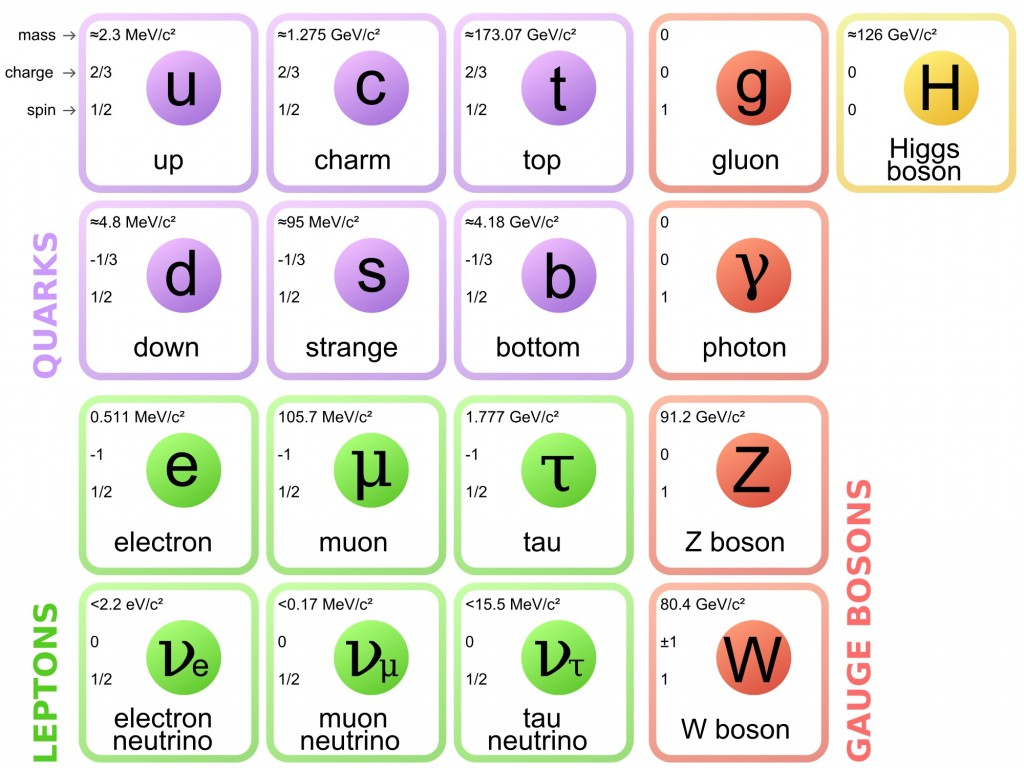
\includegraphics[width=0.75\linewidth]{figs/misc/smtable.jpg}
    \caption{
        Summary table of SM particles and their properties.
        Image taken from~\cite{THEORY:SMtableimg}.
    }
    \label{fig:smtable}
\end{figure}

Many testable predictions of the SM have been overwhelmingly validated over
the past half century, making the SM a very successful theory.
However, in addition to not accounting for gravity, there are a number
of compelling reasons to say that the SM is not a complete theory.

\FloatBarrier

\section{Beyond the standard model}

There is variety of evidence that point to beyond the SM
(BSM) physics.
A notable few concern dark matter, neutrino masses,
and the Higgs boson mass.
$\newline$

\noindent\textit{Dark matter}\newline
Astronomical observations of velocity of objects around galactic centers
have shown a clear deviation\cite{THEORY:Zwicky1933} from predictions that assume gravitational
effects only arose from matter that we can see. This is clear evidence
for the existence of ``dark'' matter (DM) which we cannot directly observe.
In fact, about 85\% of the mass in the universe is dark~\cite{THEORY:Trimble1987}.
Furthermore, DM explains observed galactic formation and 
structure as well as gravitational lensing effects~\cite{THEORY:DMstructure}.
$\newline$

\noindent\textit{Neutrino masses}\newline
The current formulation of the SM does not account for neutrino masses,
yet oscillations between neutrino flavors 
have been observed~\cite{THEORY:Fukuda1998mi},
which implies non-zero, albeit very small, neutrino masses.
$\newline$

\noindent\textit{Higgs boson mass}\newline
Because the SM does not incorporate quantum gravity,
there is an energy (or equivalently, length) scale cutoff above which we do not expect
the SM to hold. Such a cutoff, given by the Planck mass, is on the order 
of $10^{19}~\mathrm{GeV}$, approximately $10^{17}$ times larger than the electroweak scale.
We would then expect the Higgs boson mass, which recieves loop corrections from massive particles,
to be on the order of the Planck scale. However, the Higgs boson was
observed to have a mass of 125\GeV. While inelegant, this is not inherently
impossible as parameters in the theory could be ``fine-tuned'' to have
very large cancellations and result in a light Higgs boson mass.
The fine-tuning of the Higgs mass could point toward a new symmetry in the SM.
$\newline$

One popular possible solution to problems with the SM is the theory of
Supersymmetry (SUSY), which posits there is a symmetry between fermions and
bosons: each SM particle has a corresponding superpartner with spin differing
by 1/2 (fermions$~\leftrightarrow~$bosons)~\cite{THEORY:MARTIN1998}. This
must not be a perfect symmetry, otherwise we would have observed partner
particles with the same mass for the currently known SM particles. These
additional SUSY partner particles help to cancel out corrections to the Higgs
boson mass, alleviating the issue of fine-tuning (provided the masses of the
superpartners are not too much larger than the SM counterparts).


SUSY theories can be chosen to be R-parity conserving~\cite{THEORY:mohapatra2015}. That is, if $(-1)^{R} =
(-1)^{3B+L+2s}$ where $B$ is baryon number, $L$ is lepton number, and $s$ is
spin, then SM particles have $R=1$ while SUSY superpartners have $R=-1$. For
conservation of R-parity, there must be a lightest SUSY particle (LSP) which
cannot decay into two SM particles. This stable LSP is an ideal candidate for
DM if it is electrically neutral.

\section{Large Hadron Collider}

% https://twiki.cern.ch/twiki/bin/viewauth/CMS/Internal/PubDetector

We now turn to a massive machine whose 
design goal was to discover the Higgs boson and to
look for hints of (or, hopefully, discover) BSM physics
at TeV-scale energies.

This machine, the Large Hadron Collider (LHC)~\cite{LHC:Evans1129806}, is the largest and highest-energy
particle collider in the world.
Built by the European Organization
for Nuclear Research (CERN) through an international collaboration
involving over a hundred countries,
it first started operation in 2008 after a decade of construction. 
The collider resides in a tunnel with a 27-kilometer circumference,
around 100 meters below ground, and straddles the border of
France and Switzerland, near Geneva. With the help of smaller particle
accelerators situated near the LHC ring, the LHC accelerates two opposing 
beams of protons to energies of 6.5\TeV per beam and collides them by
magnetically steering the beams to cross at specified points around the ring. 
Large detectors are built around these specified point to analyze the
high energy collision products.

Proton bunches with billions of protons each are injected into the LHC ring and 
spaced apart such that bunch crossings happen up to a rate of 40 MHz.
The billions of proton-proton collisions delivered by the LHC per second
allow for many physics processes to take place. The simple formula
$N = \sigma \cdot L_\text{int}$,
gives the number of events/occurrences $N$ of a physics process
with cross-section $\sigma$ (roughly a measure of the
quantum mechanical probability of occurrence) 
in a sample of collision data with integrated luminosity
$L_\text{int}$.
The instantaneous luminosity of LHC beams
is on the order of $10^{34} \unit{cm}^{-2} \unit{s}^{-1}$.
A barn (b), the metric unit for area, is commonly used to express cross sections and luminosities,
and is equivalent to $10^{-24} \unit{cm}^2$. Thus, the LHC instantaneous luminosity can
be roughly written as $1 \unit{fb}^{-1} \unit{day}^{-1}$.
So, a potential new physics process with a cross-section of 1 fb could
manifest itself as an event in a day of collected data.
That needle would need to be found in the haystack of 
other more mundane processes. Due to the many protons per bunch,
we expect about 30 proton-proton interaction events per crossing (pileup interactions)
to disentangle from exotic signals.


\section{Compact Muon Solenoid}

The Compact Muon Solenoid (CMS)
detector~\cite{CMS:Chatrchyan2008zzk,CMS:PTDR2} is one of the general purpose
detectors situated on the LHC ring at an interaction/collision point. 
The CMS detector is 21 meters long and 15 meters tall. Its primary feature
is a 3.8 Tesla solenoidal magnet creating a magnetic field oriented along the proton 
beamline, which causes the trajectories of charged particles to bend in the plane
perpendicular to the beamline.
The detector uses layered tracking sensors and calorimeters to reconstruct the
positions and momenta of particles.

The CMS coordinate system is centered on the central collision point.
The x-axis points radially inward toward the center of the LHC,
the y-axis points vertically upward, and the z-axis points along the beamline
with the positive direction facing the west. The azimuthal angle $\phi$
around the cylindrical axis of the detector
is measured with respect to the LHC plane. The polar angle $\theta$
is measured with respect to the z-axis; however, a 
transformation of the polar angle, the pseudorapidity $\eta \equiv -\ln (\tan (\theta/2))$) 
is more commonly used
to refer to polar angles. The transverse momentum (\pt) of particles 
is measured in the x-y plane.

Let us now turn to the individual subsystems that comprise the CMS detector
starting from the center, working our way radially outward. A cutaway view of
the CMS detector, highlighting these subsystems, is shown in
Figure~\ref{fig:cmsdetector}.

\begin{figure}[!htbp]
    \centering
    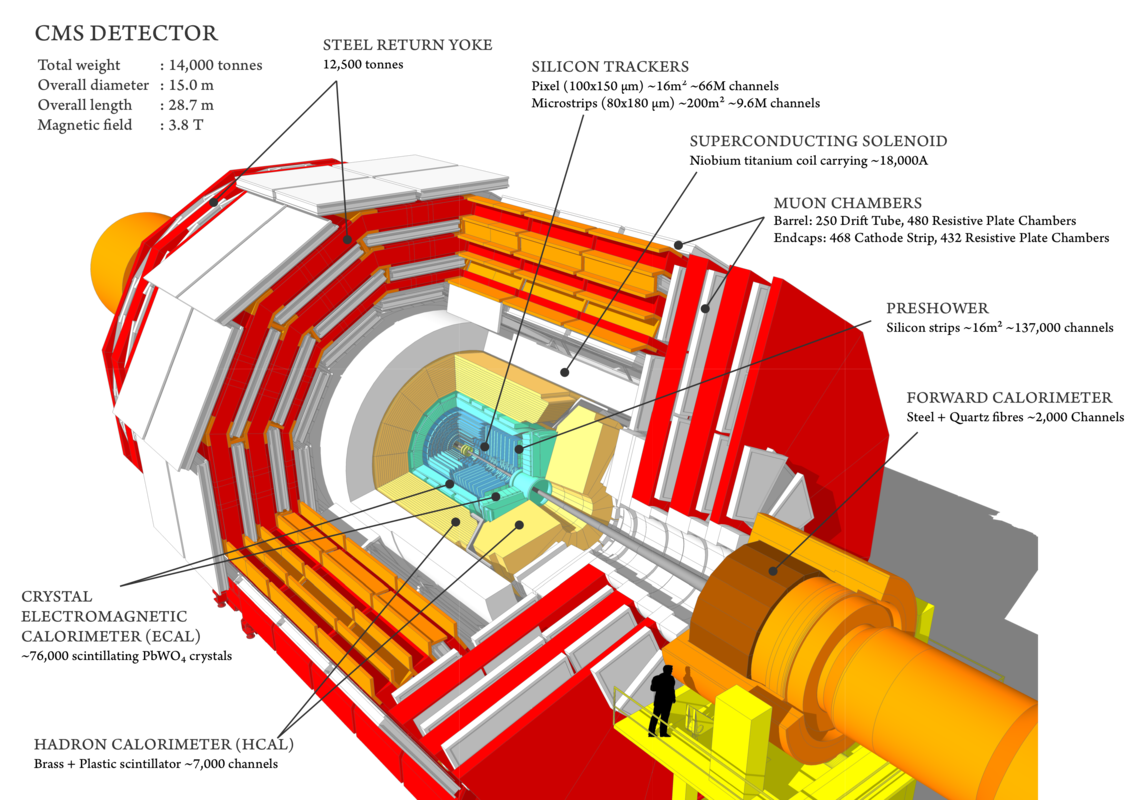
\includegraphics[width=0.99\linewidth]{figs/misc/cms.png}
    \caption{
        A cutaway view of the CMS detector.
    }
    \label{fig:cmsdetector}
\end{figure}

\FloatBarrier

\subsection{Tracker}

The innermost subdetector is the
tracker~\cite{CMS:TRK11001,CMS:Dominguez1481838}, which is composed of an
inner pixel detector and an outer strip tracker. Both use silicon technology
which allows for the formation of electron-hole pairs when a charged particle
passes through.
There are 3 layers of inner
pixel detectors with a transverse radial position ranging between $4.4\unit{cm}$ and $10.2\unit{cm}$. In 2017,
these were replaced with 4 layers ranging between $3.0\unit{cm}$ and $16.0\unit{cm}$.
The outer strip tracker consists of 10 layers in the central barrel region, extending
out to $1.1\unit{m}$. The endcaps consist of 2 disks for the inner pixel detector
and 12 disks in the strip tracker.

The tracker allows for precise reconstruction of particle trajectories and 
vertexing up to $|\eta|=2.5$ and for full range of azimuthal angles.

% % pg 15 of http://cds.cern.ch/record/1481838/files/CMS-TDR-011.pdf
% 3 layers ranging between 4.4cm and 10.2cm (2016)
% 4 layers ranging between 3.0cm and 16.0cm (2017-2018)

\subsection{Electromagnetic calorimeter}

Sitting just outside of the tracker is the electromagnetic calorimeter (ECAL).
The ECAL is composed of nearly 80,000 lead tungstate scintillating crystals tiled to form a cylinder,
and is split into a barrel section and two endcap sections~\cite{CMS:Khachatryan2015hwa}.
Together, these sections provide full azimuthal coverage and coverage up to $|\eta|=3.0$.

The high-density lead tungstate crystals, which are $22\unit{cm}$ in depth
and point toward the center of the CMS detector,
have a radiation length of $0.85\unit{cm}$. Consequently, the 25 radiation
lengths in each crystal allow electromagnetic showers to be almost completely
longitudinally contained within the single layer of crystals. The small
Moli\'ere radius of the electromagnetic showers ($2.2\unit{cm}$), 
which coincides with the
width of the crystals themselves ($2.2\unit{cm}$ in the barrel and
$2.9\unit{cm}$ in the endcaps), ensures that the transverse profile of
showers is mostly contained within just a single crystal.

\subsection{Hadronic calorimeter}

Outside of the ECAL is the hadronic calorimeter (HCAL)~\cite{CMS:PTDR2},
which is split into four sets of calorimeters to cover different geometrical
regions: barrel (HB), endcap (HE), outer (HO), and forward (HF) calorimeters.
Similar to the ECAL, the first three sections collectively coverage of hadronic showers 
up to $|\eta|=3.0$, and the HF extends the coverage to $|\eta|=5.0$.

The sampling calorimeters of the HCAL are made of alternating layers of
absorber (brass or steel) that induce hadronic showers, and plastic
scintillators. In the barrel, the brass absorbers have a total of nearly 6
interaction lengths, and along with the plastic scintillators, have
transverse segmentation with $\eta$ and $\phi$ widths of 0.087.

\subsection{Muon system}

Last, but not least, is the namesake muon system~\cite{CMS:Sirunyan2018fpa} outside of the calorimeters
and interspersed between parts of the steel return yoke. The muon system
uses three main technologies: Drift Tubes (DTs) in the barrel, Cathode
Strip Chambers (CSCs) in the endcaps, and Resistive Plate Chambers (RPCs)
in the barrel and endcaps. Together, the muon system covers up to $|\eta|=2.4$.

The barrel DTs are arranged into four stations of concentric cylinders,
and use an ionizing gas mixture of Ar/CO${}_2$ and sensitive gold-plated steel wires
to detect the ionization of throughgoing muons. Each DT has two or three layers
with wires that are either perpendicular to the beam line (to measure the $z$ coordinate),
or parallel (to measure the $\phi$ coordinate). Cylindrical stacking of
DTs provides a measurement of the $r$ coordinate.

The trapezoidal endcap CSCs cover trajectories at high-$|\eta|$. Each
detector is a multiwire proportional chamber with 6 anode wire planes alternated
with 7 cathode strip panels. Wires are oriented azimuthally and allow the measurement
of a trajectory's $r$ coordinate. Strips are oriented radially and precisely measure
the $\phi$ coordinate. CSCs provide a spatial resolution on the order of $100~\mathrm{\mu m}$.

While not as spatially precise as DTs and CSCs, the gas-filled parallel-plate RPC detectors provide excellent
time resolution (several nanoseconds) to help tag the time/bunch crossing of muon hits.

\subsection{Trigger and reconstruction}

With the extremely high rate of collisions delievered to the CMS detector by the LHC,
it is not feasible to store and reconstruct collision information for every event.
A trigger system provides a solution to this problem by evaluating if
an event is potentially useful enough to keep. This is implemented
as a two-tiered system: a Level-1 (L1) trigger and a subsequent High-Level Trigger (HLT)~\cite{CMS:Khachatryan2016bia}.

The L1 trigger stage uses custom hardware with FPGAs and look up tables to
roughly calculate various particle momenta and positions based
on information from different subdetectors
as fast as possible, in order to evaluate if an event passes specific quality
criteria. The L1 trigger reduces the event rate by a factor of a million, and is designed
to output events at less than 100 kHz.

After an event passes the L1 trigger, it is passed through the HLT stage
which is implemented in pure software and runs on a farm of computers.
Events are partially reconstructed with more precision than with the L1
stage. This HLT stage reduces the event rate to less than 1 kHz. At this point,
events are passed along to be fully reconstructed and persisted at storage facilities.

CMS uses particle-flow (PF) reconstruction algorithms~\cite{CMS:PRF14001} to
utilize information from all subdetectors to reconstruct particles within an
event. At the lowest level, particle trajectories are reconstructed from hits
in sensitive layers of detectors. Reconstruction of certain particles can
then be loosely identified with different subdetectors. For example,
electrons and photons are reconstructed with information from the tracker and
ECAL. Charged and neutral hadrons use information from the ECAL and HCAL.
Muons are reconstructed with information from the tracker and muon system.
Neutrinos are not reconstructed as they pass through the detector without
interacting, but their presence can be inferred from an imbalance of
transverse momentum in an event.
$\newline$

The remaining sections of the thesis are structured as follows.
Chapter~\ref{chap:ssdl} introduces the same-sign dilepton final state,
a promising avenue to explore new and rare physics. 
Chapter~\ref{chap:objects} discusses analysis
objects and selections for two related analyses: one is an inclusive search
for BSM, focusing on a variety of SUSY signals; the second is a SM search for the production
for four top quarks. Both utilize data delivered by the LHC
and collected by the CMS detector from 2016--2018, totaling $137$~\fbinv. 
Chapter~\ref{chap:backgrounds} describes the
SM backgrounds to these analyses. Chapter~\ref{chap:results} presents the
final results for each, and a summary with concluding remarks is given in
Chapter~\ref{chap:summary}. The results and techniques presented throughout
this thesis correspond to the published results 
in~Refs.~\cite{CMS:myTOPRun2,CMS:mySUSRun2,CMS:myTOP2016,CMS:mySUS2016}.